\documentclass[10pt,a4paper,oneside]{article}
\usepackage[brazil]{babel}
\usepackage[utf8]{inputenc}
\usepackage{amsmath}
\usepackage{amsfonts}
\usepackage{amssymb}
\usepackage[output-decimal-marker={,}]{siunitx}
\usepackage[left=3cm,right=3cm,top=2cm,bottom=2cm]{geometry}
\usepackage{hyperref} %\autoref
\usepackage{todonotes} % todos
\usepackage{placeins} %\FloatBarrier
\usepackage{caption}
\usepackage{subcaption}
\usepackage{capt-of} %Workarounds for manually inserting captions
%\usepackage{subcaption} %subfigure environment
\usepackage{xspace}
\usepackage{graphicx}
\usepackage{multirow}
\usepackage{booktabs}
\usepackage{soulutf8}
%\usepackage{titlesec} %Customization of headings


%%%%%%%%%%%% Configuring packages

\newcommand{\specialcell}[3][c]
{\begin{tabular}[#1]{@{}#2@{}}#3\end{tabular}}

\renewcommand{\thesection}{\arabic{section}}
\renewcommand{\thesubsection}{\arabic{section}.\alph{subsection}}

%%%%%%%%%%%%% Macros
\newcommand{\arat}{Aratibutantã\xspace}
\newcommand{\baep}{Baependinha\xspace}
\newcommand{\itam}{Itamaracanã\xspace}
\newcommand{\jaqu}{Jaquereçaba\xspace}
\newcommand{\para}{Paranapitanga\xspace}

\newcommand{\adm}{Administração\xspace}
\newcommand{\comp}{Computação e Matemática\xspace}
\newcommand{\edu}{Educacional\xspace}
\newcommand{\eng}{Engenharia e Produção\xspace}
\newcommand{\hum}{Humanidades\xspace}
\newcommand{\jur}{Jurídica e Contábil\xspace}

%%%%%%%%%%%%% Autor e Título

\author{%
	Alexis A. Huf, %
	Alyson D. Pereira, %
	Bruno C. N. Oliveira,\\%
	Eliza Gomes, %
	Pedro H. Penna
	}

\title{Lista de Exercícios II - Grupo 6}


\begin{document}

\maketitle

\begin{center}
	\section*{Parte 1: Distribuição Amostral da média}
\end{center}

\section{Variável Renda}
\label{questao:1}
\newcommand{\QUATROpAmostral}{\num{0.2700}\xspace}
\newcommand{\QUATROn}{200\xspace}
\newcommand{\QUATROy}{\num{54.0000}\xspace}
\newcommand{\QUATROyLinha}{\num{54.5000}\xspace}
\newcommand{\QUATROz}{\num{2.5633}\xspace}
\newcommand{\QUATROpValue}{\num{0.0052}\xspace}
\newcommand{\QUATROesVinte}{\num{0.0000}\xspace}
\newcommand{\QUATROesVinteUm}{\num{0.0248}\xspace}
\newcommand{\QUATROesVinteDois}{\num{0.0491}\xspace}
\newcommand{\QUATROesVinteTres}{\num{0.0731}\xspace}
\newcommand{\QUATROesVinteQuatro}{\num{0.0967}\xspace}
\newcommand{\QUATROesVinteCinco}{\num{0.1199}\xspace}
\newcommand{\QUATROesVinteSeis}{\num{0.1428}\xspace}
\newcommand{\QUATROesVinteSete}{\num{0.1655}\xspace}
\newcommand{\QUATROpVinte}{\num{0.0100}\xspace}
\newcommand{\QUATROpVinteUm}{\num{0.0241}\xspace}
\newcommand{\QUATROpVinteDois}{\num{0.0514}\xspace}
\newcommand{\QUATROpVinteTres}{\num{0.0980}\xspace}
\newcommand{\QUATROpVinteQuatro}{\num{0.1687}\xspace}
\newcommand{\QUATROpVinteCinco}{\num{0.2641}\xspace}
\newcommand{\QUATROpVinteSeis}{\num{0.3797}\xspace}
\newcommand{\QUATROpVinteSete}{\num{0.5057}\xspace}
\newcommand{\QUATROesAmostra}{\num{0.0731}\xspace}
\newcommand{\QUATROtamanhoAmostra}{\num{4055.1080}\xspace}
\newcommand{\QUATROtamanhoAmostraRounded}{4056\xspace}


Foram retiradas 200 amostras, sem reposição, com tamanhos 4, 8, 16, 30 e 100, 
dentre os 4986 alunos que possuíam um valor definido para a variável Renda.
A população possuí média $\mu$ = ${\UMx}$ para a variável Renda, com desvio padrão $\sigma$ = ${\UMsd}$.
A \autoref{tab:q1} apresentam os valores da média e desvio padrão para cada tamanho
de amostra e seu respectivo valor esperado de desvio padrão.

\begin{table}[h]
\centering
\caption{Valores das médias amostrais para a variável \textit{Renda}}
\label{tab:q1}
\vspace{0.5em}
\begin{tabular}{l r r r}
	\toprule
	\textbf{\specialcell{c}{Tamanho da\\Amostra}} & \textbf{Média} & \textbf{\specialcell{c}{Desvio\\Padrão}} & \textbf{$\frac{\sigma}{\sqrt{n}}$}\\
	\midrule
	$4$       & ${\UMxQuatro}$   & ${\UMsdQuatro}$   & ${\UMsdeQuatro}$   \\
	$8$       & ${\UMxOito}$   & ${\UMsdOito}$   & ${\UMsdeOito}$   \\
	$16$      & ${\UMxDezesseis}$  & ${\UMsdDezesseis}$  & ${\UMsdeDezesseis}$  \\
	$30$      & ${\UMxTrinta}$  & ${\UMsdTrinta}$  & ${\UMsdeTrinta}$  \\
	$100$     & ${\UMxCem}$ & ${\UMsdCem}$ & ${\UMsdeCem}$ \\
	\bottomrule
\end{tabular}
\end{table}

\subsection{Valor esperado da média amostral}
Na \autoref{tab:q1} é possível observar que a medida que se aumenta o tamanho da amostra o valor da média fica cada vez mais próximo ao valor da média populacional, que é de ${\UMx}$.


\subsection{Valor esperado do desvio padrão da média amostral}
Conforme indicado na \autoref{tab:q1}, os valores de desvio padrão das amostras ficam mais próximos aos valores de $\frac{\sigma}{\sqrt{n}}$ à medida que se aumenta o tamanho das amostras.

\subsection{Distribuição amostral da média}
Conforme indicado nas \autoref{fig:m4,fig:m8,fig:m16,fig:m30,fig:m100}, a medida que se aumenta o tamanho da amostra,
a distribuição amostral se torna similar a uma distribuição normal.

\begin{figure}[h]
\begin{minipage}{0.50\textwidth}
	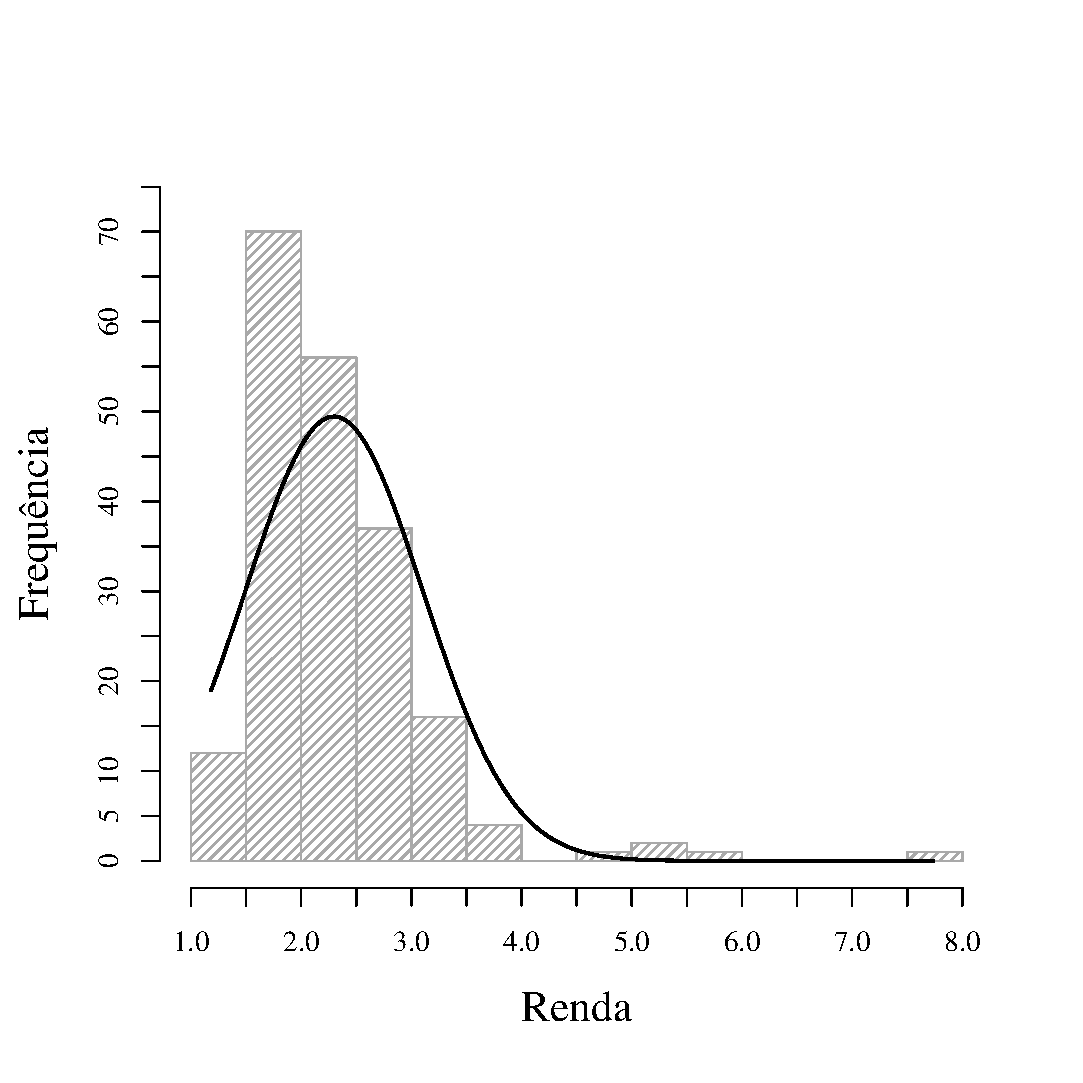
\includegraphics[width=\linewidth]{plots/histogram_renda_n4.eps}
	\caption{Amostra de tamanho 4}
	\label{fig:m4}
\end{minipage}
\begin{minipage}{0.50\textwidth}
	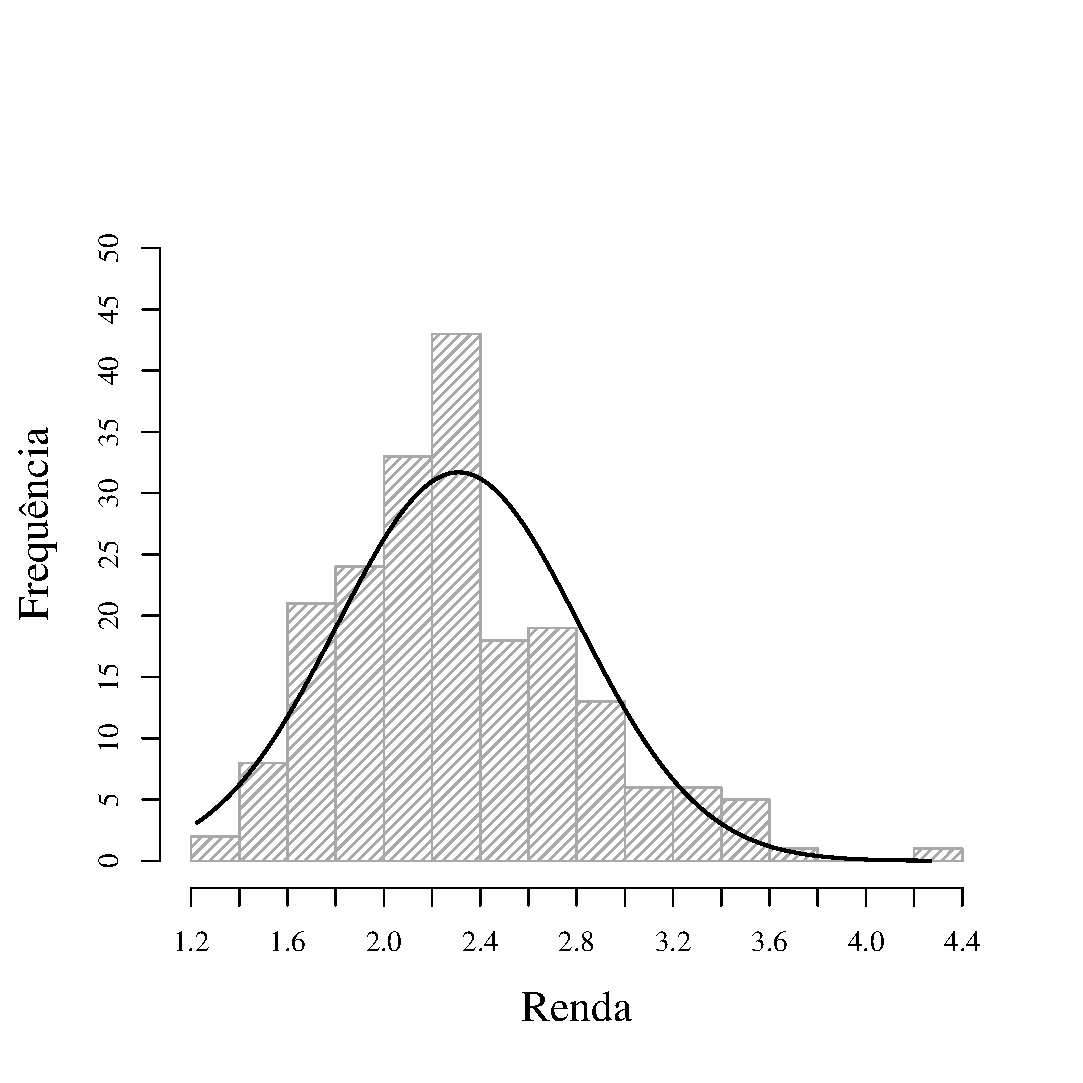
\includegraphics[width=\linewidth]{plots/histogram_renda_n8.eps}
	\caption{Amostra de tamanho 8}
	\label{fig:m8}
\end{minipage}
\end{figure}

\begin{figure}[h]
\begin{minipage}{0.50\textwidth}
	\includegraphics[width=\linewidth]{plots/histogram_renda_n16.eps}
	\caption{Amostra de tamanho 16}
	\label{fig:m16}
\end{minipage}
\begin{minipage}{0.50\textwidth}
	\includegraphics[width=\linewidth]{plots/histogram_renda_n30.eps}
	\caption{Amostra de tamanho 30}
	\label{fig:m30}
\end{minipage}
\end{figure}

\begin{figure}[h]
\centering
	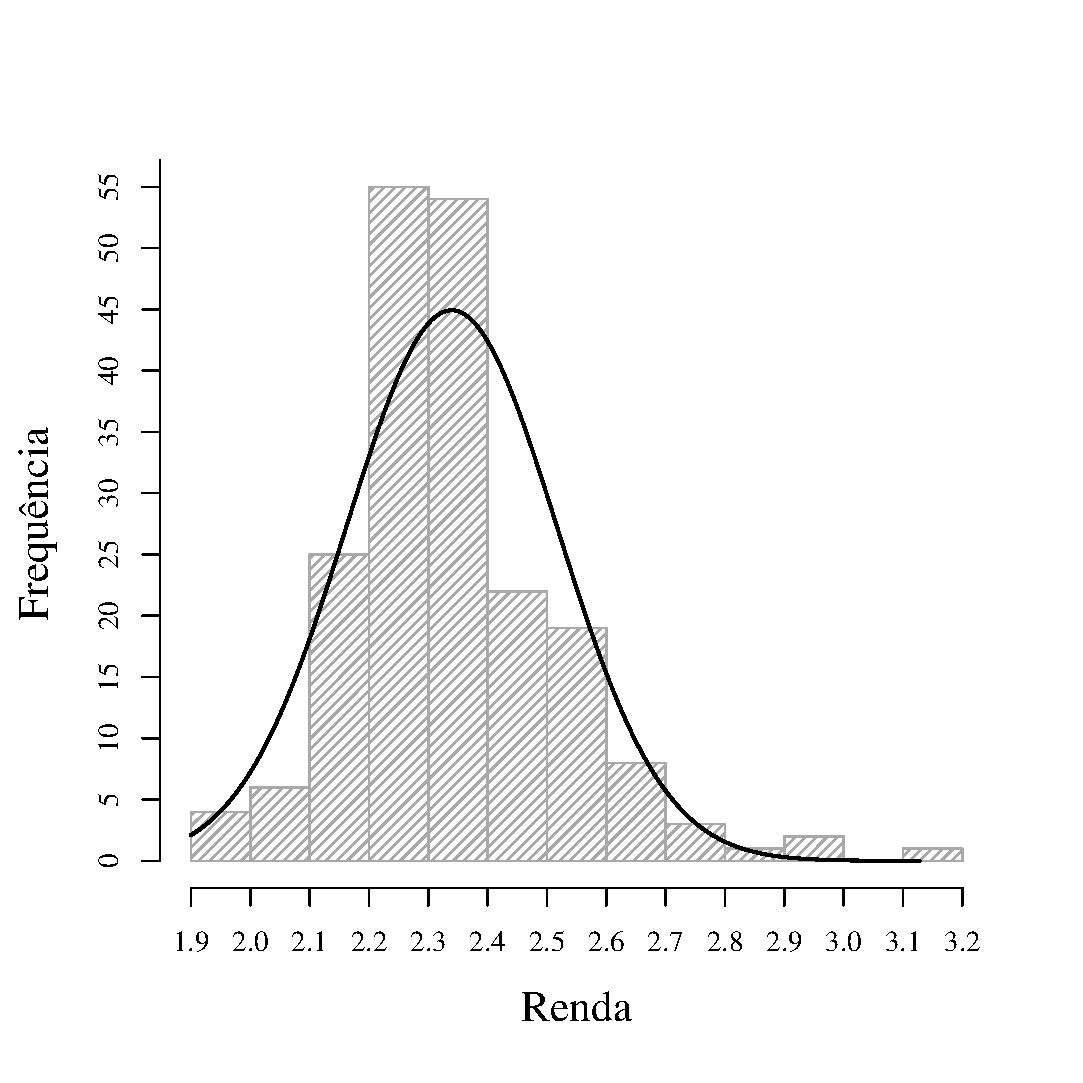
\includegraphics[width=0.50\textwidth]{plots/histogram_renda_n100.eps}
	\caption{Amostra de tamanho 100}
	\label{fig:m100}
\end{figure}

\FloatBarrier


\begin{center}
	\section*{Parte 2: Intervalos de Confiança para Média}
\end{center}

\section{Variável Idade}
\label{questao:2}
\subsection{Intervalo de 95\% de confiança para a média populacional da Idade dos alunos}
\label{sub:1a}
	
	Após retirar os dados perdidos da variável Idade, foi retirada uma
	amostra aleatória de 20 alunos, dos quais a variável idade foi obtida por meio de sorteio. Com a amostra
	adquirida, tem-se média $\bar{x}$ = \num{32,1} e desvio padrão s = \num{4,930037}.
	Com o desvio padrão da população desconhecido, utiliza-se o desvio
	padrão da amostra ($s = \num{4,930037}$).  O tamanho da população é conhecido ($N
	= 4987$) e o da amostra é pequeno, $n < 50$, então, nesse caso utiliza-se
	a distribuição t de Student.

	Para obter o intervalo de confiança para a média em uma população
	conhecida, é possível utilizar a seguinte equação:

	
	\begin{align}
		\label{eq:dois-a-expr}
		IC (\mu, \gamma) = \bar{x} \pm t_\gamma \frac{s}{\sqrt{n}} \sqrt{\frac{N-n}{N-1}}
	\end{align}

	Para um intervalo de confiança de 95\%, obtém-se o valor da cauda
	superior de \num{0,025}. Diante disso, procura-se na tabela da distribuição
	t de student o grau de liberdade 19, pois gl = n-1, e o valor \num{0,025},
	resultando em $t = \num{2,093}$. Inserindo os valores na equação
	tem-se:

	\begin{align*}
		IC (\mu, 95\%) &= \num{32,1} \pm \num{2,093} \frac{\num{4,930037}}{\sqrt{20}} \sqrt{\frac{4987 - 20}{4987 - 1}} \\
		IC (\mu, 95\%) &= \num{32,1} \pm \num{2,3024}
	\end{align*}

	A média de idades de amostra é \num{32,1} anos, com o nível de confiança de
	95\%, a margem de erro é de \num{2,3024} anos para mais ou para menos. Diante
	disso, o intervalo de confiança é de [\num{29,7976}; \num{34,4024}].

\subsection{Intervalo de 99\% de confiança para a média populacional da Idade dos alunos, com uma precisão de 2 anos}

	\todo[inline]{(...) utiliza-se da amostra piloto com $n=20$, o desvio (...)}
    \todo[inline]{Mesma coisa sobre $t$ de Student para $n \leq 50$}
	Com o desvio padrão da população desconhecido, utiliza-se como amostra
	piloto n = 20 e desvio padrão $s = \num{6,11534}$, obtidos anteriormente. Como o
	tamanho da amostra é pequeno ($n < 30$) utiliza-se a
	distribuição t student.

	Para saber o tamanho da amostra necessário para estimar a média
	populacional da idade dos alunos, com erro amostral máximo tolerado de 2
	anos, utiliza-se a seguinte equação:

	\begin{align}
		\label{eq:dois-b-expr1}
		 n_0 = \left (\frac{t_\gamma s}{E_0} \right)^2
	\end{align}

	Sabendo-se que o grau de liberdade é 19, pois gl = n - 1, e o nível de
	confiança é de 99\%, o valor da cauda superior será de \num{0,005}. Obtendo os
	valores da tabela de distribuição t student, t = \num{2,861}.
	Inserindo os valores na equação, tem-se:

    \todo[inline]{No livro arredondamento do $n_0$ só acontece quando ele é atribuído pra $n$. Acho que aqui $\cong 77$ não faz sentido, já que ali embaixo, $n_0$ é usado como \num{76.52}}
	\begin{align*}
		n_0 = \left (\frac{\num{2,861} \times \num{6,11534}}{2} \right)^2 = \num{76,52} \cong 77
	\end{align*}

	Como o tamanho da população não é grande e é conhecido, adicionalmente,
	utiliza-se a seguinte equação para calcular o tamanho da amostra.

	\begin{align}
		\label{eq:dois-b-expr2}
		n = \frac{N . n_0}{N + n_0}
	\end{align}

	Inserindo os valores na equação, tem-se:

	\begin{align*}
		n &= \Big\lceil \frac{4987 \times \num{76,52}}{4987 + \num{76,52}} \Big\rceil \\
		n &= \lceil \num{75,3636} \rceil \\
		n &= 76
	\end{align*}

	Diante dos cálculos apresentados acima, pode-se dizer que uma amostra
	com 20 elementos não é suficiente para encontrar um intervalo de 99\% de
	confiança para a média populacional da idade dos alunos com um erro
	máximo tolerado de 2 anos. Seriam necessários, no mínimo $76$ elementos da
	amostra para garantir certa precisão. 

\subsection{Você concorda com o plano de amostragem usado, que considerou a população homogênea}
	
	\todo[inline]{\st{Com o objetivo de caracterizar melhor o perfil dos alunos através da
	variável idade, o}O plano de amostragem (...)}
    \todo[inline]{(...) uma vez que \hl{uma análise exploratória dos dados da população} mostra que a variável idade (...)}
    %Eliza, avacalhei com tuas quebras de linhas quando troquei \textquotedblleft e 
    %\textquotedblright por ``''. Você não tinha um apego emocional nal com elas, tinha?
	Com o objetivo de caracterizar melhor o perfil dos alunos através da
	variável idade, o plano de amostragem utilizado, considerando a
	população homogênea, não é o ideal, uma vez que a variável idade está
	associada a pelo menos uma outra variável. Por exemplo, existe uma
	associação entre a variável Idade e a variável Opinião, mostrando que os
	alunos com idades inferiores a 30 anos possuem maiores percentuais
	(\num{72,57}\%) para a opinião `` Muito Satisfeitos'', enquanto os 
    alunos com idades superiores
	a 30 anos possuem maiores percentuais (\num{25,62}\%) para a opinião
    `` Indiferente'', não obtendo flutuação
	maior do que 5\% para as opiniões ``Satisfeitos'' (\num{21,94}\%) 
    e ``Insatisfeitos'' (\num{21,28}\%). Além disso, o perfil dos
	alunos pode ser analisado através da associações entre outras variáveis,
	como por exemplo, Opinião e Pagamento e Pagamento e Região, conforme
	apresentado na Lista 1. 

	Como resultado da associação entre Opinião e Pagamento, observou-se que
	os alunos que pagam sua mensalidade com Auxílio de Familiares são mais
	`` Indiferentes'' (\num{36,96}\%), com Bolsas
	de Estudos são mais `` Indiferentes''
	(\num{38,72}\%), com Financiamento Bancário são mais ``Muito Satisfeitos''
    (\num{66,36}\%), com Incentivos Federal são mais``Insatisfeitos'' (\num{35,30}\%) e com
	Recursos Próprios são mais ``
	Satisfeitos'' (\num{34,48}\%).

	Por outro lado, a associação entre as variáveis Pagamento e Região
	apresentou o seguinte resultado: os alunos de Aratibutantã utilizam,
	maioritariamente, a forma de pagamento por ``Incentivos Federais''
    (\num{47,51}\%), os de Baependinha utilizam o
	`` Financiamento Bancário'' (\num{53,01}\%), os
	de Itamaracanã utilizam o `` Financiamento Bancário'' 
    (\num{90,98}\%), os de Jaquereçaba utilizam os
	`` Incentivos Federais'' (\num{76,68}\%) e por
	fim, os alunos de Paranapitanga utilizam, maioritariamente, a forma de
	pagamento `` Incentivos Federais'' (\num{95,87}\%). 

	Para caracterizar melhor o perfil dos alunos, poderia ser realizado um
	plano de amostragem estratificada proporcional, uma vez que se conhece,
	neste caso, as características da população (quantos e quais são os
	tamanhos dos estratos). 


\section{Variável Renda}
\label{questao:3}
\newcommand{\QUATROpAmostral}{\num{0.2700}\xspace}
\newcommand{\QUATROn}{200\xspace}
\newcommand{\QUATROy}{\num{54.0000}\xspace}
\newcommand{\QUATROyLinha}{\num{54.5000}\xspace}
\newcommand{\QUATROz}{\num{2.5633}\xspace}
\newcommand{\QUATROpValue}{\num{0.0052}\xspace}
\newcommand{\QUATROesVinte}{\num{0.0000}\xspace}
\newcommand{\QUATROesVinteUm}{\num{0.0248}\xspace}
\newcommand{\QUATROesVinteDois}{\num{0.0491}\xspace}
\newcommand{\QUATROesVinteTres}{\num{0.0731}\xspace}
\newcommand{\QUATROesVinteQuatro}{\num{0.0967}\xspace}
\newcommand{\QUATROesVinteCinco}{\num{0.1199}\xspace}
\newcommand{\QUATROesVinteSeis}{\num{0.1428}\xspace}
\newcommand{\QUATROesVinteSete}{\num{0.1655}\xspace}
\newcommand{\QUATROpVinte}{\num{0.0100}\xspace}
\newcommand{\QUATROpVinteUm}{\num{0.0241}\xspace}
\newcommand{\QUATROpVinteDois}{\num{0.0514}\xspace}
\newcommand{\QUATROpVinteTres}{\num{0.0980}\xspace}
\newcommand{\QUATROpVinteQuatro}{\num{0.1687}\xspace}
\newcommand{\QUATROpVinteCinco}{\num{0.2641}\xspace}
\newcommand{\QUATROpVinteSeis}{\num{0.3797}\xspace}
\newcommand{\QUATROpVinteSete}{\num{0.5057}\xspace}
\newcommand{\QUATROesAmostra}{\num{0.0731}\xspace}
\newcommand{\QUATROtamanhoAmostra}{\num{4055.1080}\xspace}
\newcommand{\QUATROtamanhoAmostraRounded}{4056\xspace}

Foi retirada uma amostra aleatória simples, sem reposição, com 20 elementos,
dentre os \TRESN alunos que possuíam um valor definido para a variável Renda.
A população possui média \TRESX e desvio padrão de \TRESSD.
A média amostral obtida foi de \TRESx com desvio padrão de \TRESsd.

\subsection{Intervalo de 95\% de confiança para a média populacional da Renda dos alunos}
Como o tamanho da amostra é pequeno (n < 30), devemos calcular o intervalo
de confiança utilizando a \textit{distribuiçao t de Student}. Para um intervalo
de confiança de 95\% e 19 graus de liberdade, obtemos um valor t = 2.093.
Assim, podemos calcular o intervalo de confiança de acordo com a \autoref{eq:dois-a-expr}:

\begin{align*}
	IC (\mu, 95\%) &= \TRESx \pm 2.093 \frac{\TRESsd}{\sqrt{\TRESn}} \sqrt{\frac{\TRESN - \TRESn}{\TRESN - 1}} \\
	IC (\mu, 95\%) &= \TRESx \pm \TRESdelta
\end{align*}

Assim, o intervalo de (\TRESicmin;\TRESicmax) contêm, com 95\% confiança, o
valor da média populacional para a variável Renda.

\subsection{Intervalo de 99\% de confiança para a média populacional da Renda dos alunos}
Para um intervalo de confiança de 99\% e 19 graus de liberdade, obtemos um valor t = 2.861.
Utilizando novamente a \autoref{eq:dois-a-expr}:

\begin{align*}
	IC (\mu, 99\%) &= \TRESx \pm 2.861 \frac{\TRESsd}{\sqrt{\TRESn}} \sqrt{\frac{\TRESN - \TRESn}{\TRESN - 1}} \\
	IC (\mu, 99\%) &= \TRESx \pm \TRESdeltaNoveNove
\end{align*}

Assim, o intervalo de \TRESicNoveNoveMin à \TRESicNoveNoveMax contêm, com grau de confiança de 99\%, o valor
da média populacional para a variável Renda. Nota-se que o intervalo ficou maior em relação ao intervalo com grau de confiança de 95\%. Para diminuir esse intervalo seria necessário aumentar o tamanho da amostra.

\subsection{Tamanho mínimo da amostra para um intervalo de 99\% de confiança e precisão de 1.5 salários}
Para se obter o tamanho mínimo da amostra, primeiramente utilizamos a \autoref{eq:dois-b-expr1}:

\begin{align*}
	n_0 = \left (\frac{2.861 \times \TRESsd}{1.5} \right)^2 = \TRESnZero \cong \TRESnZeroRounded
\end{align*}

Como tamanho da população não é grande e é conhecido, adicionalmente utilizamos a \autoref{eq:dois-b-expr2}. Assim:

\begin{align*}
		n &= \lceil \frac{\TRESN \times \TRESnZero}{\TRESN + \TRESnZero} \rceil \\
		n &= \lceil \TRESnZeroCorrigido \rceil \\
		n &= \TRESnZeroCorrigidoRounded
\end{align*}

Portanto, são necessários \TRESnZeroCorrigidoRounded amostras para se obter, com 99\% de confiança,
um intervalo com precisão de 1.5 salários mínimos.


\newpage
\begin{center}
	\section*{Parte 3: Intervalos de Confiança para Proporção}
\end{center}

	Nas questões que se seguem, são estudados os intervalos de confiança
	para a proporção de algumas das variáveis da população. Para fins de
	síntese, considere as seguintes equações no desenvolvimento dessa
	terceira parte.
	
	A estimação do parâmetro proporção da população foi feita com base na
	Equação \ref{equation: intervalo de confianca para proporcao 1}.

		\begin{equation}
			IC(p, \gamma) = \hat{p} \pm z_\gamma \sigma_{\hat{p}}
			\label{equation: intervalo de confianca para proporcao 1}
		\end{equation}
	
	Alternativamente, quando $\sigma_{\hat{p}}$ não é conhecido, e $n$ é
	suficientemente grande ($n \geq 50$), $\sigma_{\hat{p}}$ pode
	ser aproximado por $s_{\hat{p}}$, o desvio padrão da amostra tomada, e o
	parâmetro proporção pode ser estimado de acordo com a Equação
	\ref{equation: intervalo de confianca para proporcao 2}.

		\begin{equation}
			IC(p, \gamma) = \hat{p} \pm z_\gamma \sqrt{\frac{\hat{p}(1-\hat{p})}{n}} \\
			\label{equation: intervalo de confianca para proporcao 2}
		\end{equation}
	
	O cálculo do tamanho de uma amostra necessária para que $|\hat{p} - p|
	\leq E_0$ é feito de acordo com a Equação \ref{equation: tamanho amostra
	1} e a Equação \ref{equation: tamanho amostra 2}.

	\begin{equation}
		n_0 = \frac{z_\gamma^2 p(1-p)}{E_0^2}
		\label{equation: tamanho amostra 1}
	\end{equation}

	\begin{equation}
		n = \frac{N n_0}{N + n_0 - 1}
		\label{equation: tamanho amostra 2}
	\end{equation}

	Por fim, poara se obter o erro amostral máximo, dado o tamanho da
	amostra, a Equação \eqref{eq:quatro-b-e0-expr} e a Equação
	\eqref{eq:quatro-b-n0-expr} são empregradas. Sabemos $n$, $N$, $z\gamma$
	e $\hat{p}$, que pode ser usado para aproximar $p$. Para encontrar
	$E_0$, podemos deduzir \eqref{eq:quatro-b-e0-expr} algebricamente de
	\eqref{eq:quatro-b-n0}.  Para encontrar $n_0$, usado em
	\eqref{eq:quatro-b-e0-expr}, $n_0$ pode ser
	isolada\footnote{\url{https://www.wolframalpha.com/input/?i=solve+n\%3D(N*m)\%2F(N\%2Bm-1)+for+m}}
	em \eqref{eq:quatro-b-n}, resultando em \eqref{eq:quatro-b-n0-expr}. 

	\begin{equation}
		E_0 = \label{eq:quatro-b-e0-expr}
			   \sqrt{\frac{z_\gamma p(1 - p) }{n_0}} \\
	\end{equation}

	\begin{equation}
		n_0 = \label{eq:quatro-b-n0-expr}
			   \frac{n-n N}{n-N} \qquad \forall (n, N) : n \neq N
	\end{equation}

\section{Variável Pagamento}
\label{questao:4}
\newcommand{\QUATROpAmostral}{\num{0.2700}\xspace}
\newcommand{\QUATROn}{200\xspace}
\newcommand{\QUATROy}{\num{54.0000}\xspace}
\newcommand{\QUATROyLinha}{\num{54.5000}\xspace}
\newcommand{\QUATROz}{\num{2.5633}\xspace}
\newcommand{\QUATROpValue}{\num{0.0052}\xspace}
\newcommand{\QUATROesVinte}{\num{0.0000}\xspace}
\newcommand{\QUATROesVinteUm}{\num{0.0248}\xspace}
\newcommand{\QUATROesVinteDois}{\num{0.0491}\xspace}
\newcommand{\QUATROesVinteTres}{\num{0.0731}\xspace}
\newcommand{\QUATROesVinteQuatro}{\num{0.0967}\xspace}
\newcommand{\QUATROesVinteCinco}{\num{0.1199}\xspace}
\newcommand{\QUATROesVinteSeis}{\num{0.1428}\xspace}
\newcommand{\QUATROesVinteSete}{\num{0.1655}\xspace}
\newcommand{\QUATROpVinte}{\num{0.0100}\xspace}
\newcommand{\QUATROpVinteUm}{\num{0.0241}\xspace}
\newcommand{\QUATROpVinteDois}{\num{0.0514}\xspace}
\newcommand{\QUATROpVinteTres}{\num{0.0980}\xspace}
\newcommand{\QUATROpVinteQuatro}{\num{0.1687}\xspace}
\newcommand{\QUATROpVinteCinco}{\num{0.2641}\xspace}
\newcommand{\QUATROpVinteSeis}{\num{0.3797}\xspace}
\newcommand{\QUATROpVinteSete}{\num{0.5057}\xspace}
\newcommand{\QUATROesAmostra}{\num{0.0731}\xspace}
\newcommand{\QUATROtamanhoAmostra}{\num{4055.1080}\xspace}
\newcommand{\QUATROtamanhoAmostraRounded}{4056\xspace}


	Foi retirada uma amostra aleatória simples, sem reposição, com \QUATROn
	elementos, dentre os \QUATRON alunos que possuíam um valor definido para a
	variável Pagamento. A proporção amostral $\hat{p}$ de alunos cuja fonte de
	Pagamento era ``Incentivos Federais'' foi de \QUATROpAmostral.

\subsection{Intervalo de confiança}

	O intervalo de confiança para a proporção $p$ é dado pela
	\autoref{eq:quatro-a-expr}.

	\begin{align} 
		IC(p, 95\%) \label{eq:quatro-a-expr}
					&= \hat{p} \pm z_\gamma \sigma_{\hat{p}} \\
					\label{eq:quatro-a-estim}
					&= \hat{p} \pm z_\gamma \sqrt{\frac{\hat{p}(1-\hat{p})}{n}} \\
					&= \QUATROpAmostral \pm \QUATROzy \sqrt{\frac{\QUATROpAmostral (1- \QUATROpAmostral)}{\QUATROn}} \nonumber \\
					&= \QUATROpAmostral \pm \QUATROAdelta \nonumber \\
					\label{eq:quatro-a-result}
					&= [\QUATROAICinf, \QUATROAICsup]
	\end{align}

	Dada uma amostra aleatória simples de \QUATROn alunos tomados dentre os
	\QUATRON da população, há 95\% de chance de que a proporção amostral $\hat{p}$ 
    de alunos cuja fonte de recursos são ``Incentivos Federais'' seja um valor 
    contido no intervalo \eqref{eq:quatro-a-result}.

	Em \eqref{eq:quatro-a-expr}, $\sigma_{\hat{p}}$ simboliza o desvio
	padrão de $\hat{p}$ em todas as amostras aleatórias que podem ser
	tomadas da população. Como não possuímos tal parâmetro (que depende da 
    proporção populacional $p$), e como $n$ é grande ($n = \QUATROn \geq 50$),
    $\sigma_{\hat{p}}$ foi aproximado por $s_{\hat{p}}$, o desvio padrão da 
    amostra tomada.

\subsection{Precisão}

	No contexto dessa questão, é possível calcular o tamanho da amostra
	necessária para que $|\hat{p} - p| \leq E_0$ usando as fórmulas
	\eqref{eq:quatro-b-n0} e \eqref{eq:quatro-b-n}.

	\begin{align}
		n_0 &= \label{eq:quatro-b-n0}
			   \frac{z_\gamma^2 p(1-p)}{E_0^2} \\
		n &= \label{eq:quatro-b-n}
			 \frac{N n_0}{N + n_0 - 1} 
	\end{align}

	Para obter o erro amostral máximo, dado o tamanho da amostra, as
	equações \eqref{eq:quatro-b-e0-expr} e \eqref{eq:quatro-b-n0-expr} podem
	ser usadas. Sabemos $n$, $N$, $z\gamma$ e $\hat{p}$, que pode ser usado para
	aproximar $p$. Para encontrar $E_0$, podemos deduzir
	\eqref{eq:quatro-b-e0-expr} algebricamente de \eqref{eq:quatro-b-n0}.
	Para encontrar $n_0$, usado em \eqref{eq:quatro-b-e0-expr}, $n_0$ pode
	ser isolada\footnote{\url{https://www.wolframalpha.com/input/?i=solve+n\%3D(N*m)\%2F(N\%2Bm-1)+for+m}}
    em \eqref{eq:quatro-b-n}, resultando em
	\eqref{eq:quatro-b-n0-expr}. 

	\begin{align}
		E_0 &= \label{eq:quatro-b-e0-expr}
			   \sqrt{\frac{z_\gamma p(1 - p) }{n_0}} \\
		n_0 &= \label{eq:quatro-b-n0-expr}
			   \frac{n-n N}{n-N} \qquad \forall (n, N) : n \neq N
	\end{align}

	Combinando \eqref{eq:quatro-b-e0-expr} e \eqref{eq:quatro-b-n0-expr} e
	substituindo os valores, o erro amostral máximo de uma amostra com
	\QUATROn elementos é dado por \eqref{eq:quatro-b-e0-calc}.

	\begin{align}
		\label{eq:quatro-b-e0-calc}
		E_0 &= \sqrt{\frac{z_\gamma \hat{p}(1 - \hat{p}) }{\frac{n-n N}{n - N}}} \\
			&= \sqrt{\frac{\QUATROzy \;\cdot\; \QUATROpAmostral (1 - \QUATROpAmostral) }{\frac{\QUATROn - \QUATROn \;\cdot\; \QUATRON}{\QUATROn - \QUATRON}}} \nonumber \\
			&= \QUATROBE \nonumber
	\end{align}

	Como $E_0 = \QUATROBE$, a amostra não é suficiente para uma margem de
	erro de 2\%. Usando \eqref{eq:quatro-b-n0} obtemos $n_0$ necessário para
	uma margem de erro de 2\% em \eqref{eq:quatro-b-n0-result}.
	% e \eqref{eq:quatro-b-n} (pois sabemos o tamanho da população),
	% necessitaríamos de uma amostra com \QUATROBn elementos. Os detalhes
	% são mostrados em \eqref{eq:quatro-b-n-2p}.

	\begin{align}
		n_0 &= \frac{z_\gamma^2 p(1-p)}{E_0^2} \nonumber \\
			&= \frac{\QUATROzy^2 \cdot \QUATROpAmostral(1-\QUATROpAmostral)}{\num{0.02}^2} \nonumber \\
			&= \label{eq:quatro-b-n0-result}
			   \QUATROBnz	
	\end{align}

	Como o tamanho da população é conhecido, o valor em
	\eqref{eq:quatro-b-n0-result} pode ser reduzido para o valor em
	\eqref{eq:quatro-b-n-result}.

	\begin{align}
		n &= \Big\lceil \frac{N n_0}{N + n_0 - 1} \nonumber \Big\rceil \\
		  &= \lceil \QUATROBn \nonumber \rceil \\
		  &= \label{eq:quatro-b-n-result} \QUATROBnceil
	\end{align}

\subsection{Tamanho da amostra sem amostra piloto}

	Para estimar o tamanho da amostra que garanta erro amostral máximo de
	2\% sem uma estimativa adequada para a proporção populacional $p$, deve
	ser utilizada a fórmula \eqref{eq:quatro-c-n0-expr} para obtenção de
	$n_0$. A fórmula em \eqref{eq:quatro-c-n0-expr} foi obtida
	superestimando $p$ como $\num{0.5}$ e aplicando isso em \eqref{eq:quatro-b-n0}

	\begin{align}
		n_0 &= \label{eq:quatro-c-n0-expr}
			   \frac{z_\gamma^2 \cdot \num{0.5} \cdot (1 - \num{0.5})}{E_0^2} = \frac{z_\gamma^2}{4 \cdot E_0^2} \\
			&= \frac{\QUATROzy^2}{4 \cdot (\num{0.02})^2} \nonumber \\
			&= \label{eq:quatro-c-n0-result}
			   \QUATROCnz
	\end{align}

	Novamente, \eqref{eq:quatro-c-n0-result} pode ser substituído em
	\eqref{eq:quatro-b-n}, resultando no tamanho da amostra necessário, em
	\eqref{eq:quatro-c-n-result}.

	\begin{align}
		n &= \Big\lceil \frac{N n_0}{N + n_0 - 1} \nonumber \Big\rceil \\
		  &= \Big\lceil \frac{\QUATRON \cdot \QUATROCnz}{\QUATRON + \QUATROCnz -1} \nonumber \Big\rceil \\
		  &= \lceil \QUATROCn \nonumber \rceil \\
		  &= \label{eq:quatro-c-n-result} 
			 \QUATROCnceil
	\end{align}

	Portanto, considerando a ausência de uma amostra piloto, é preciso ter
	uma amostra de tamanho mínimo de \QUATROCnceil para estimar com 95\% de
	confiança e precisão de 2\% a proporção populacional de alunos de EAD da
	TYU que usam incentivos federais.


\section{Variável Opinião}
\label{questao:5}
\subsection{Diferença entre as Médias}

Sabe-se que o tamanho da população é $N = 4850$ e os valores obtidos da amostra de 80 elementos são apresentados na Tab. \ref{tb:5a}.

\begin{table}[ht]
\centering
\caption{Valores de Tamanho da Amostra, Média e Desvio-Padrão} 
\label{tb:5a}
\begin{tabular}{cccc}
  \toprule
  Pagamento C & n & $\bar{x}$ & s \\
  \midrule
 Incentivos Federais & 28 & 3.6560 & 1.4513 \\ 
 Outras Formas de Pagamento & 52 & 1.8305 & 0.7834 \\
   \bottomrule
\end{tabular}
\end{table}

Como a variância populacional é desconhecida, primeiramente, faz-se necessário determinar estatisticamente se as variâncias dos dois grupos são iguais ou diferentes. Para isso, são formuladas as 
seguintes hipóteses:

\begin{align*} 
		H_0\!:   &\; \sigma^2_1 = \sigma^2_2 \\
		H_1\!:   &\; \sigma^2_1 \neq \sigma^2_2  \\
		\alpha\!:&\; 0.01
\end{align*}

Para comparar as variâncias, com nível de significância de $1\%$, foi realizado o teste f com o seguinte código no programa R.

\inputr{questao5/5a1.R}

Foram passados como parâmetros para o teste f as rendas dos alunos que pagam suas mensalidades com incentivos federais (\r|incentivos\$Renda|), as rendas dos alunos que pagam suas mensalidades com 
outras formas de pagamento (\r|outras\$Renda|), a indicação de que se trata de um teste bilateral (\r|alternative = two.sided|), nível de confiança de 99\% (\r|conf.level = 0.99|).

Com a execução do código, o R retornou o $valor-p = 0.0001465$, o que permite rejeitar $H_{0}$. Considerando que o $valor-p$ é menor do que a significância ($\alpha = 0.01$), pode-se dizer que há 
evidências estatísticas que as variâncias são diferentes. Com isso, é possível determinar se há diferença entre as médias dos dois grupos.  

Para determinar a diferença, ou não, entre as médias das variáveis Incentivos Federais e Outras Formas de Pagamento, primeiramente faz-se necessário determinar as hipóteses:

\begin{align*} 
		H_0\!:   &\; \mu_1 = \mu_2 \\
		H_1\!:   &\; \mu_1 \neq \mu_2  \\
		\alpha\!:&\; 0.05
\end{align*}

onde $H_{0}$ representa as igualdades entre as médias e $H_{1}$ a diferença entre elas. De acordo com as hipóteses, pode-se dizer que se trata de um teste bilateral.

Para testar as médias foi realizado o teste t utilizando o programa R com o seguinte código:

\inputr{questao5/5a.R}

A variável \textquotedblleft amostra\textquotedblright representa a amostra de 80 elementos. Foram passados como parâmetros para o teste t as rendas dos alunos que pagam suas mensalidades com 
incentivos federais (\r|incentivos\$Renda|), as rendas dos alunos que pagam suas mensalidades com outras formas de pagamento (\r|outras\$Renda|), a indicação de que se trata de um teste bilateral 
(\r|alternative = two.sided|), nível de confiança de 95\% (\r|conf.level = 0.95|) e que as variâncias são diferentes (\r|var.equal = FALSE|).

Com a execução do código, o R retornou o $valor-p = 0.0000004046$. Como a significância é $\alpha = 0.05$ e $valor-p < \alpha$, rejeita-se $H_{0}$ e conclui-se que: há evidências estatísticas que as 
médias das rendas dos alunos que pagam suas mensalidades com \textquotedblleft Incentivos Federais\textquotedblright e as dos alunos que pagam suas mensalidades com \textquotedblleft Outras 
Formas de Pagamento\textquotedblright são diferentes. 

\subsection{Poder do Teste}

Para obter o desvio agrupado a partir dos desvios padrões e tamanho de cada subgrupo é preciso calcular a variância agregada, utilizando a equação \ref{eq:5b}.

\begin{equation}
 \label{eq:5b}
 S^2_a = \frac{(n_1 - 1) \cdot S^2_1 + (n_2 - 1) \cdot S^2_2}{n_1 + n_2 - 2}
\end{equation}

Substituindo os valores tem-se:

\begin{align*}
 S^2_a &\; = \frac{(28 - 1) \cdot 1.4513^2 + (52 - 1) \cdot 0.7834^2}{28 + 52 - 2} \\
       &\; = 1.1303 \\
\end{align*}

Tirando a raiz quadrada, tem-se o valor do desvio padrão da amostra de acordo com o tamanho das amostras dos dois grupos. Nesse caso, $S_a = 1.0631$ salários mínimos.

Para calcular o poder do teste, foi utilizado o programa R com o seguinte código:

\inputr{questao5/5b.R}

A variável $tempD$ representa o valor da variável de teste ($\bar{x} / S_a$), na qual o valor $-10$ irá variar para $-5$, $-2$, $-1$, $1$, $2$, $5$, $10$. A variável $n$ representa a quantidade de 
elementos da amostra, $d$ a diferença entre as médias medida em números de desvios padrões, $sig. level$ o nível de significância ($5\%$), $power$ o poder do teste, $type$ determina que são duas 
amostras independentes e $alternative$ que é um teste bilateral.

A Tabela \ref{tb:5b} apresenta os dados obtidos com a execução do código descrito acima.

\begin{table}[ht]
\centering
\caption{Poder do teste para diferença entre as médias das rendas dos alunos} 
\label{tb:5b}
\begin{tabular}{cccc}
  \toprule
  & & \multicolumn{2}{c}{$1 - \beta$} \\
  \cline{3-4}
  Diferenças entre as médias & Diferenças / $S_a$  & $n = 28$ & $n = 52$ \\
  \midrule
 $-10$ & $9.4064$ & $1$ & $1$ \\ 
 $-5$  & $4.7032$ & $1$ & $1$ \\
 $-2$  & $1.8812$ & $0.9999$ & $1$ \\
 $-1$  & $0.9406$ & $0.9327$ & $0.9973$ \\
 $1$   & $0.9406$ & $0.9327$ & $0.9973$ \\
 $2$   & $1.8812$ & $0.9999$ & $1$ \\
 $5$   & $4.7032$ & $1$ & $1$ \\
 $10$  & $9.4064$ & $1$ & $1$ \\
   \bottomrule
\end{tabular}
\end{table}

Pode-se observar que, de acordo com os dados, conforme a diferença entre as duas médias aumenta o poder do teste também aumenta, independentemente de qual lado.

\subsection{Tamanho Mínimo de Amostra}

Para obter o tamanho mínimo da amostra utilizou-se o programa R com o seguinte código:

\inputr{questao5/5c.R}

A Tabela \ref{tb:5c} apresenta os resultados obtidos pelo programa.

\begin{table}[ht]
\centering
\caption{Poder do teste para diferença entre as médias das rendas dos alunos} 
\label{tb:5c}
\begin{tabular}{cccc}
  \toprule
  Diferenças entre as médias & Tamanho da Amostra & Diferenças / $S_a$  & $1 - \beta$ \\
  \midrule
 $3$ & $6.3732$ & $2.8219$ & $0.95$ \\ 
   \bottomrule
\end{tabular}
\end{table}

Conforme pode ser analisado, o tamanho da amostra coletada é suficiente para detectar, com 95\% de probabilidade e 1\% de significância, que a diferença entre as médias das rendas dos alunos que 
pagam suas mensalidades com Incentivos Federais e dos alunos que pagam com Outras Formas de Pagamento é de 3 salários mínimos, visto que $n \approx 7$ elementos.


\section{Variável Renda}
\label{questao:6}
\newcommand{\QUATROpAmostral}{\num{0.2700}\xspace}
\newcommand{\QUATROn}{200\xspace}
\newcommand{\QUATROy}{\num{54.0000}\xspace}
\newcommand{\QUATROyLinha}{\num{54.5000}\xspace}
\newcommand{\QUATROz}{\num{2.5633}\xspace}
\newcommand{\QUATROpValue}{\num{0.0052}\xspace}
\newcommand{\QUATROesVinte}{\num{0.0000}\xspace}
\newcommand{\QUATROesVinteUm}{\num{0.0248}\xspace}
\newcommand{\QUATROesVinteDois}{\num{0.0491}\xspace}
\newcommand{\QUATROesVinteTres}{\num{0.0731}\xspace}
\newcommand{\QUATROesVinteQuatro}{\num{0.0967}\xspace}
\newcommand{\QUATROesVinteCinco}{\num{0.1199}\xspace}
\newcommand{\QUATROesVinteSeis}{\num{0.1428}\xspace}
\newcommand{\QUATROesVinteSete}{\num{0.1655}\xspace}
\newcommand{\QUATROpVinte}{\num{0.0100}\xspace}
\newcommand{\QUATROpVinteUm}{\num{0.0241}\xspace}
\newcommand{\QUATROpVinteDois}{\num{0.0514}\xspace}
\newcommand{\QUATROpVinteTres}{\num{0.0980}\xspace}
\newcommand{\QUATROpVinteQuatro}{\num{0.1687}\xspace}
\newcommand{\QUATROpVinteCinco}{\num{0.2641}\xspace}
\newcommand{\QUATROpVinteSeis}{\num{0.3797}\xspace}
\newcommand{\QUATROpVinteSete}{\num{0.5057}\xspace}
\newcommand{\QUATROesAmostra}{\num{0.0731}\xspace}
\newcommand{\QUATROtamanhoAmostra}{\num{4055.1080}\xspace}
\newcommand{\QUATROtamanhoAmostraRounded}{4056\xspace}


Para avaliação da variável Renda, primeiramente foi feita uma recodificação
da mesma em uma variável qualitativa de dois valores: alunos com renda
familiar inferior a $\num{2,5}$ salários mínimos e alunos com renda igual ou
superior a $\num{2,5}$ salários mínimos. Nesse processo, apenas foram considerados
aqueles alunos que possuíam um valor definido para a variável, totalizando
$N=\SEISN$ alunos. Em seguida, retirou-se uma amostra aleatória simples de
\SEISn elementos dessa população. A proporção amostral $\hat{p}$ de alunos
com renda superior a $\num{2.5}$ salários mínimos é de \SEISpAmostral.

\subsection{Intervalo de Confiança}

	Como $\sigma_{\hat{p}}$ não é conhecido e $n$ é suficientemente grande,
	o intervalo de confiança para a proporção $p$ foi calculado pela
	\autoref{equation: intervalo de confianca para proporcao 2}.
	%
	\begin{align*}
		IC(p, 95\%) &= \SEISpAmostral \pm \SEISzy \sqrt{\frac{\SEISpAmostral (1- \SEISpAmostral)}{\SEISn}} \\
		IC(p, 95\%) &= \SEISpAmostral \pm \SEISAdelta \\
		IC(p, 95\%) &= [\SEISAICinf, \SEISAICsup]
	\end{align*}

	Dada uma amostra aleatória simples de \SEISn alunos
	selecionados dentre os \SEISN da população há $95\%$ de chance de que a
	proporção de alunos que possuem renda familiar superior a $\num{2,5}$ salários
	mínimos seja um valor no intervalo $[\SEISAICinf, \SEISAICsup]$

\subsection{Precisão}

	O erro amostral máximo de uma amostra com \SEISn elementos é dado pela
	Equação \ref{equation: erro amostral maximo}.
	%
	\begin{align*}
		E_0 &= \sqrt{\frac{\SEISzy \;\cdot\; \SEISpAmostral (1 - \SEISpAmostral) }{\frac{\SEISn - \SEISn \;\cdot\; \SEISN}{\SEISn - \SEISN}}} \\
		E_0 &= \SEISBE
	\end{align*}

	Como $E_0 = \SEISBE$, a amostra não é suficiente para uma margem de erro
	de 2\%. Usando a Equação \ref{equation: tamanho amostra 1} obtemos o
	valor de $n_0$ necessário para uma margem de erro de 2\%:

	\begin{align*}
		n_0 &= \frac{\SEISzy^2 \cdot \SEISpAmostral(1-\SEISpAmostral)}{\num{0.02}^2} \\
		n_0 &= \SEISBnz
	\end{align*}

	Como o tamanho da população é conhecido, esse valor pode ser reduzido
	para, aplicando-se a Equação \ref{equation: tamanho amostra 2}.

	\begin{align*}
		n &= \Big\lceil \frac{\SEISN \cdot  \SEISBnz}{\SEISN + \SEISBnz - 1} \Big\rceil \\
		  &= \lceil \SEISBn \rceil \\
		  &= \SEISBnceil
	\end{align*}


\subsection{Tamanho da Amostra sem Amostra-Piloto}

	Para se estimar o tamanho da amostra que um garanta erro amostral máximo de
	2\% sem uma estimativa adequada para a proporção populacional $p$, é
	feita uma super estimação da Equação \ref{equation: tamanho amostral
	maximo} com $p = 0.5$.
	%
	\begin{align*}
		n_0 &= \frac{z_\gamma^2 \cdot \num{0.5} \cdot (1 - \num{0.5})}{E_0^2} \\
		n_0 &= \frac{z_\gamma^2}{4 \cdot E_0^2} \\
		n_0 &= \frac{\SEISzy^2}{4 \cdot (\num{0.02})^2} \\
		n_0 &= \SEISCnz
	\end{align*}

	Usando esse valor para $n_0$ superestimado, pode-se calcular o tamanho da
	amostra necessária pela Equação \ref{equation: tamanho amostra 2}.
	%
	\begin{align*}
		n &= \Big\lceil \frac{\SEISN \cdot \SEISCnz}{\SEISN + \SEISCnz - 1} \Big\rceil \\
		n &= \lceil \SEISCn \rceil \\
		n &= \SEISCnceil
	\end{align*}

	Portanto, considerando a ausência de uma amostra piloto, é preciso ter uma
	amostra de tamanho mínimo de \SEISCnceil para estimar com 95\% de
	confiança e precisão de 2\% a proporção populacional de alunos de EAD da TYU
	apresentam renda familiar superior a $\num{2,5}$ salários mínimos.

\subsection{Impactos na Recodificação da Variável}
	
	A recodificação de uma varíavel quantitativa em uma qualitativa sempre
	resulta em perda de informação. Por isso, para a análise do intervalo de
	confiança para o parâmetro média da variável \textit{Renda}, o mais
	indicado seria que a estimação fosse feita com a variável original.

	No entanto, é interessante ressaltar que o intervalo de confiança se
	aplica ao parâmetro sendo estimado. Portanto, caso o intuito seja
	estudar o parâmetro proporção, a recodificação se faz necessária para a
	variável \textit{Renda}.


\end{document}
